
\block{Introdução}
{
	As balanças foram criadas por necessidade durante o desenvolvimento de comercio na antiguidade, os produtos que não recorriam a contagem por unidades, tais como objetos irregulares por exemplo o ouro tinham de se quantificar seu valor, e a forma de medir sua massa tornou-se numa variável de medição para troca de bens. A relíquia mais antiga de uma balança de medir massa foi descoberto na vila de Indus River, perto do conhecido por hoje de Pakistão, e estima-se ser por volta de 2000 B.C.
	Estas primeiras balanças eram alavancas em equilíbrio [ F1 × b1c = F2 × b2c ], onde nos extremos eram colocados cestos e se colocava os pesos, este estava centrado no seu centro de massa, assim se os pesos nos dois cestos serem iguais fica em equilíbrio (na horizontal), era um sistema de comparar com pesos ?xos estabelecidos como norma (contra-pesos).
	
	Os métodos de medir a massa de objetos não conheceu nenhumas melhorias tecnológicas relevantes até a era industrial. Só nos anos do século XVIII é que o meio de medir a massa de objetos não dependia de contra-pesos. As balanças por molas foi inventado por Richard Salter, um fabricante de balanças por volta dos anos de 1770 na Inglaterra.
	
	O que vai ser utilizado no projeto vai ser um célula de peso que seque o principio acima mencionado, estes sensores tem quatro strain gauges ligadas em ponte wheatstone que vão detetar a distorção (pressão) do material, ou seja, a célula de peso e gerar um sinal em tensão proporcional a força exercida. Seque o mesmo principio de uma mola [ $K= \frac{\Delta l}{F}$ ].
}
\begin{columns}
	\column{0.4}
	\block{More text}{Text and more text}
	
	\column{0.6}
	\block{Something else}{Here, \blindtext \vspace{4cm}}
	\note[
	targetoffsetx=-9cm, 
	targetoffsety=-6.5cm, 
	width=0.5\linewidth
	]
	{e-mail \texttt{welcome@overleaf.com}}
\end{columns}

\begin{columns}
	\column{0.1}
	\column{0.8}
	\block{Kit Desenvolvimento}
	{
		\begin{tikzfigure}
			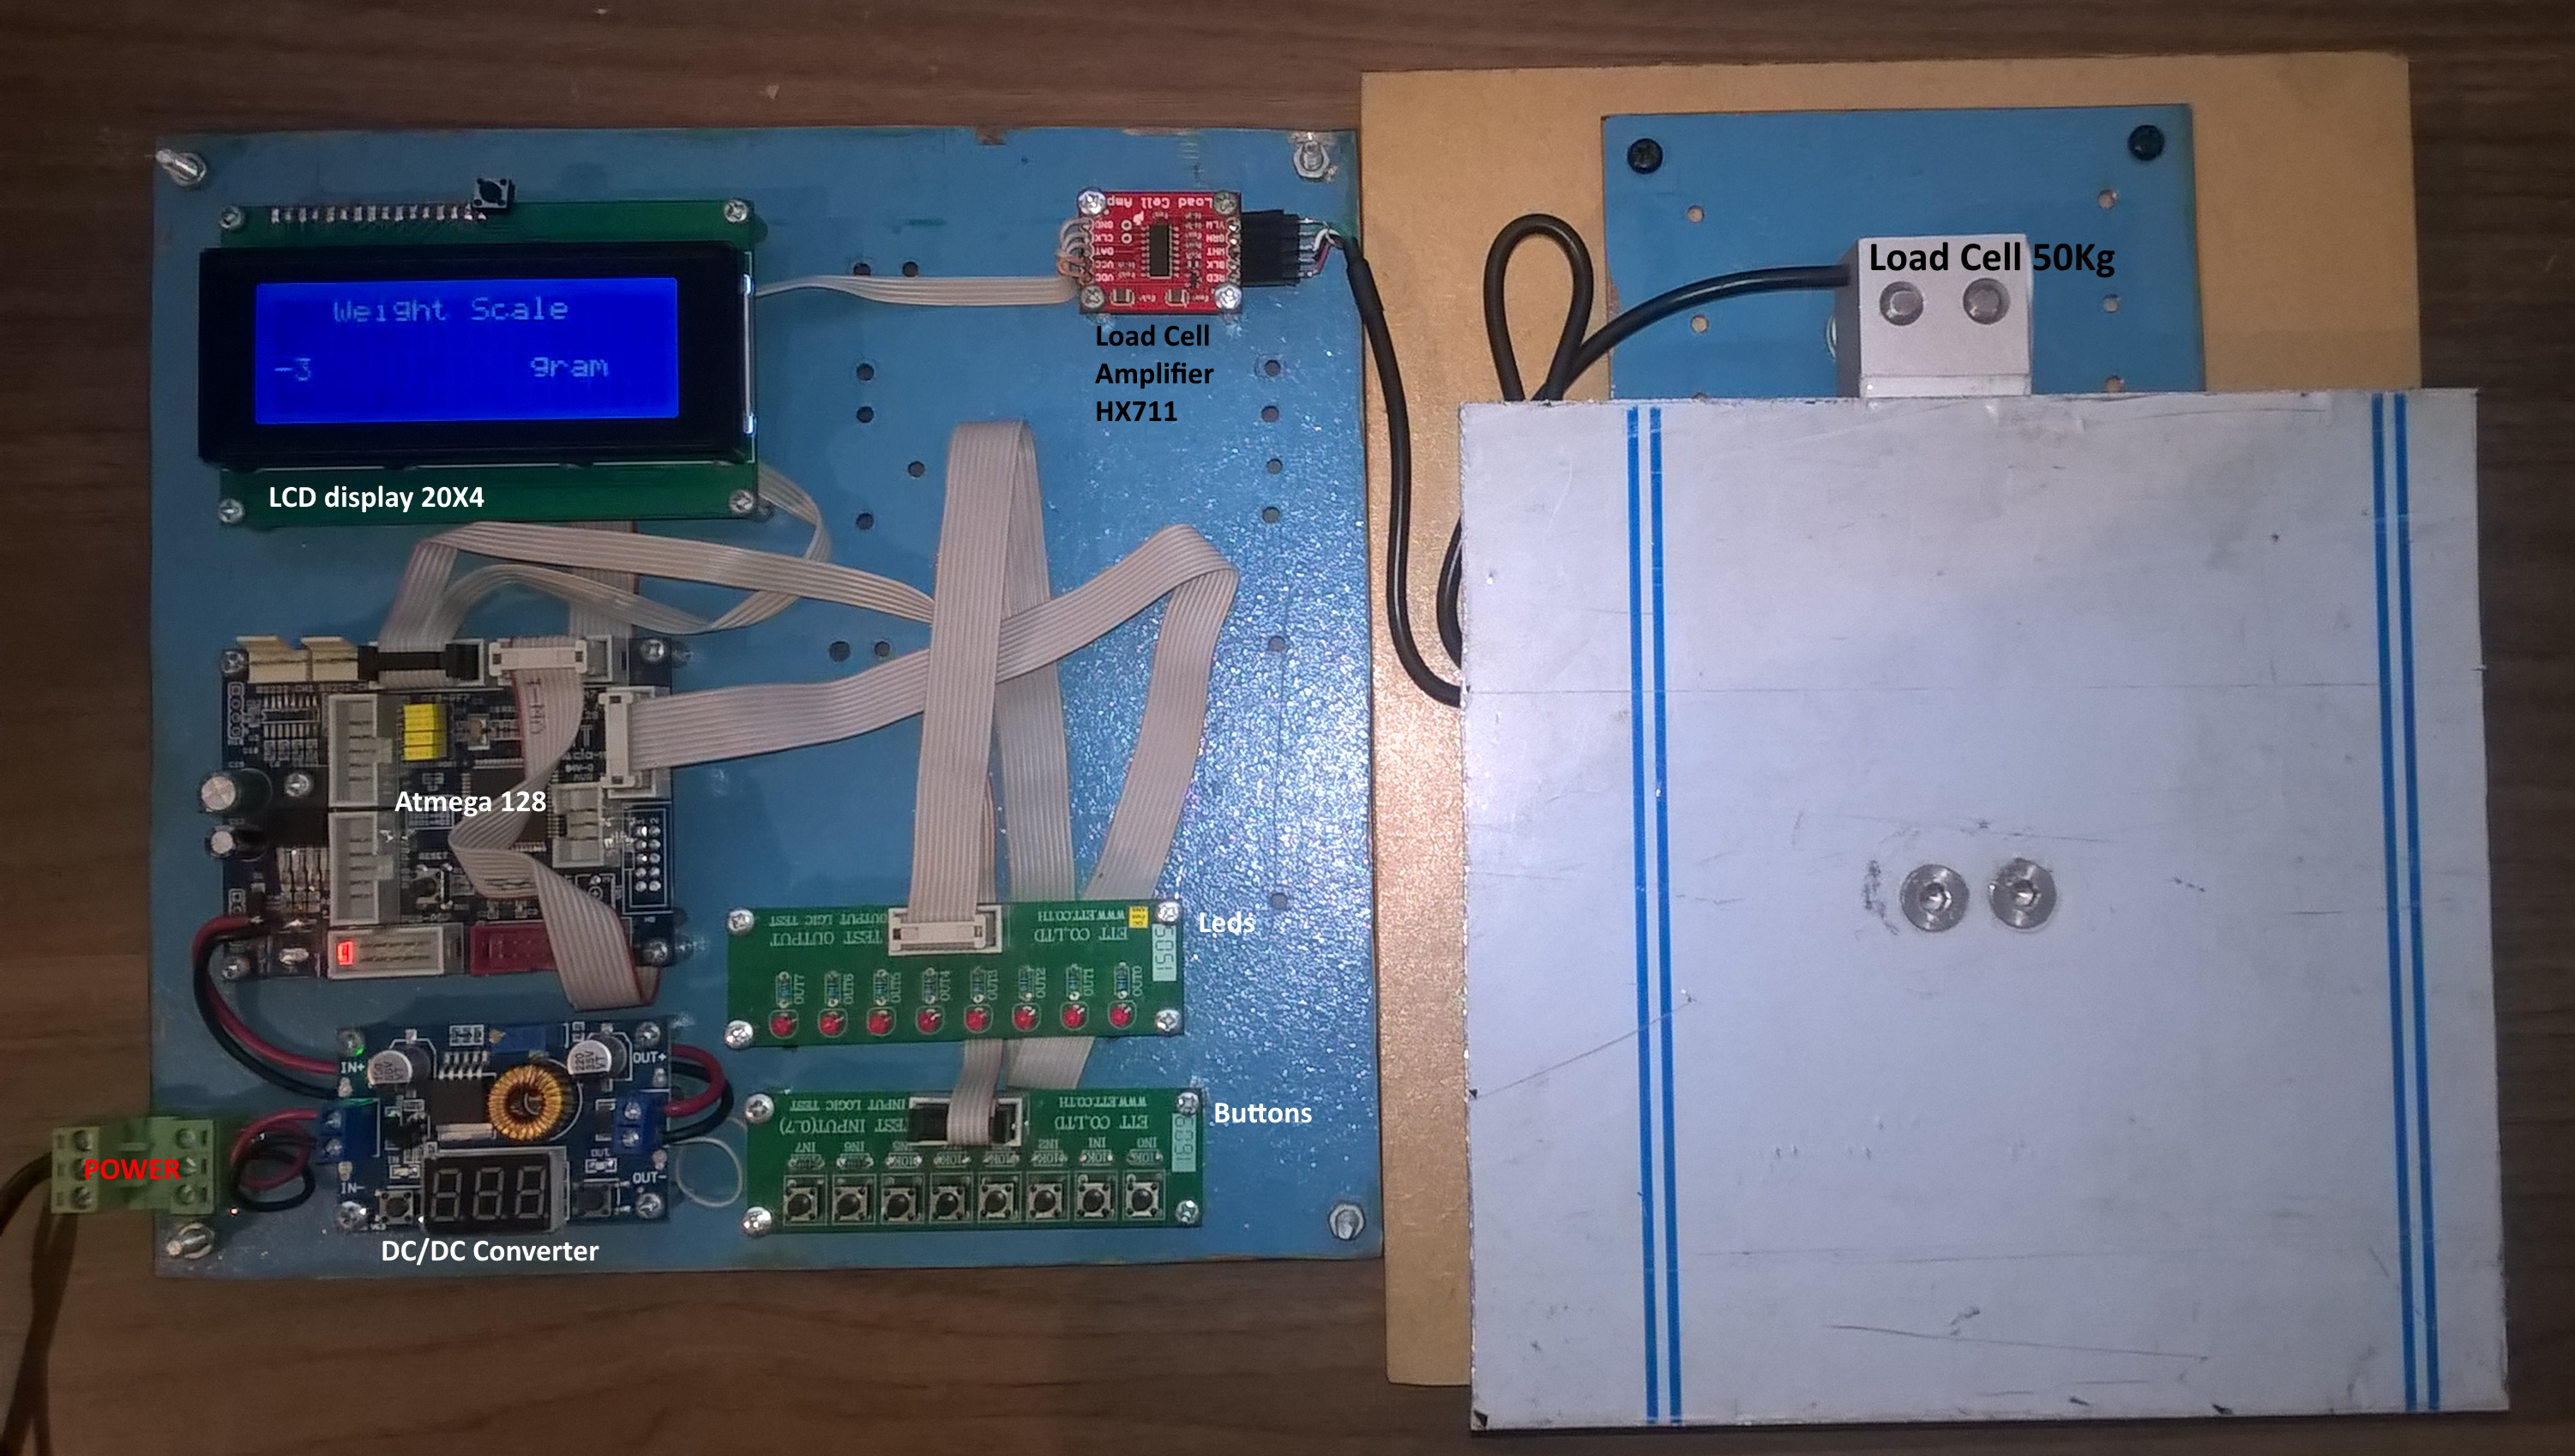
\includegraphics[width=0.7\textwidth]{./image/PESTA/kit/Kit_Desenvolvimento_2.jpg}
		\end{tikzfigure}
	}
	%\column{0.5}
	%\block{Description of the figure}{\blindtext}
\end{columns}

\column{.65}
\block{More Examples of LateX}{
\bigskip
you can even put stuff in color boxes.\\
\coloredbox{
	\begin{itemize}
		\item 1
		\item 2
	\end{itemize}
\lipsum[2]
\bigskip

\innerblock{here is some math}{

\begin{center}
$2^5+5x-\frac{}{}*3=7$
\end{center}
}
}	
}
\block{More text}{\lipsum[1]}
\column{.35}
\block{more pictures}{

\includegraphics[width=\linewidth]{./image/PESTA/ISEP_marca_cor_grande.png}
\lipsum[4]

}
\block{the end}{\lipsum[10-11]}


